\section{Используемые технологии}
\subsection{Модель CUDA}
\begin{figure}[h]
    \centering
    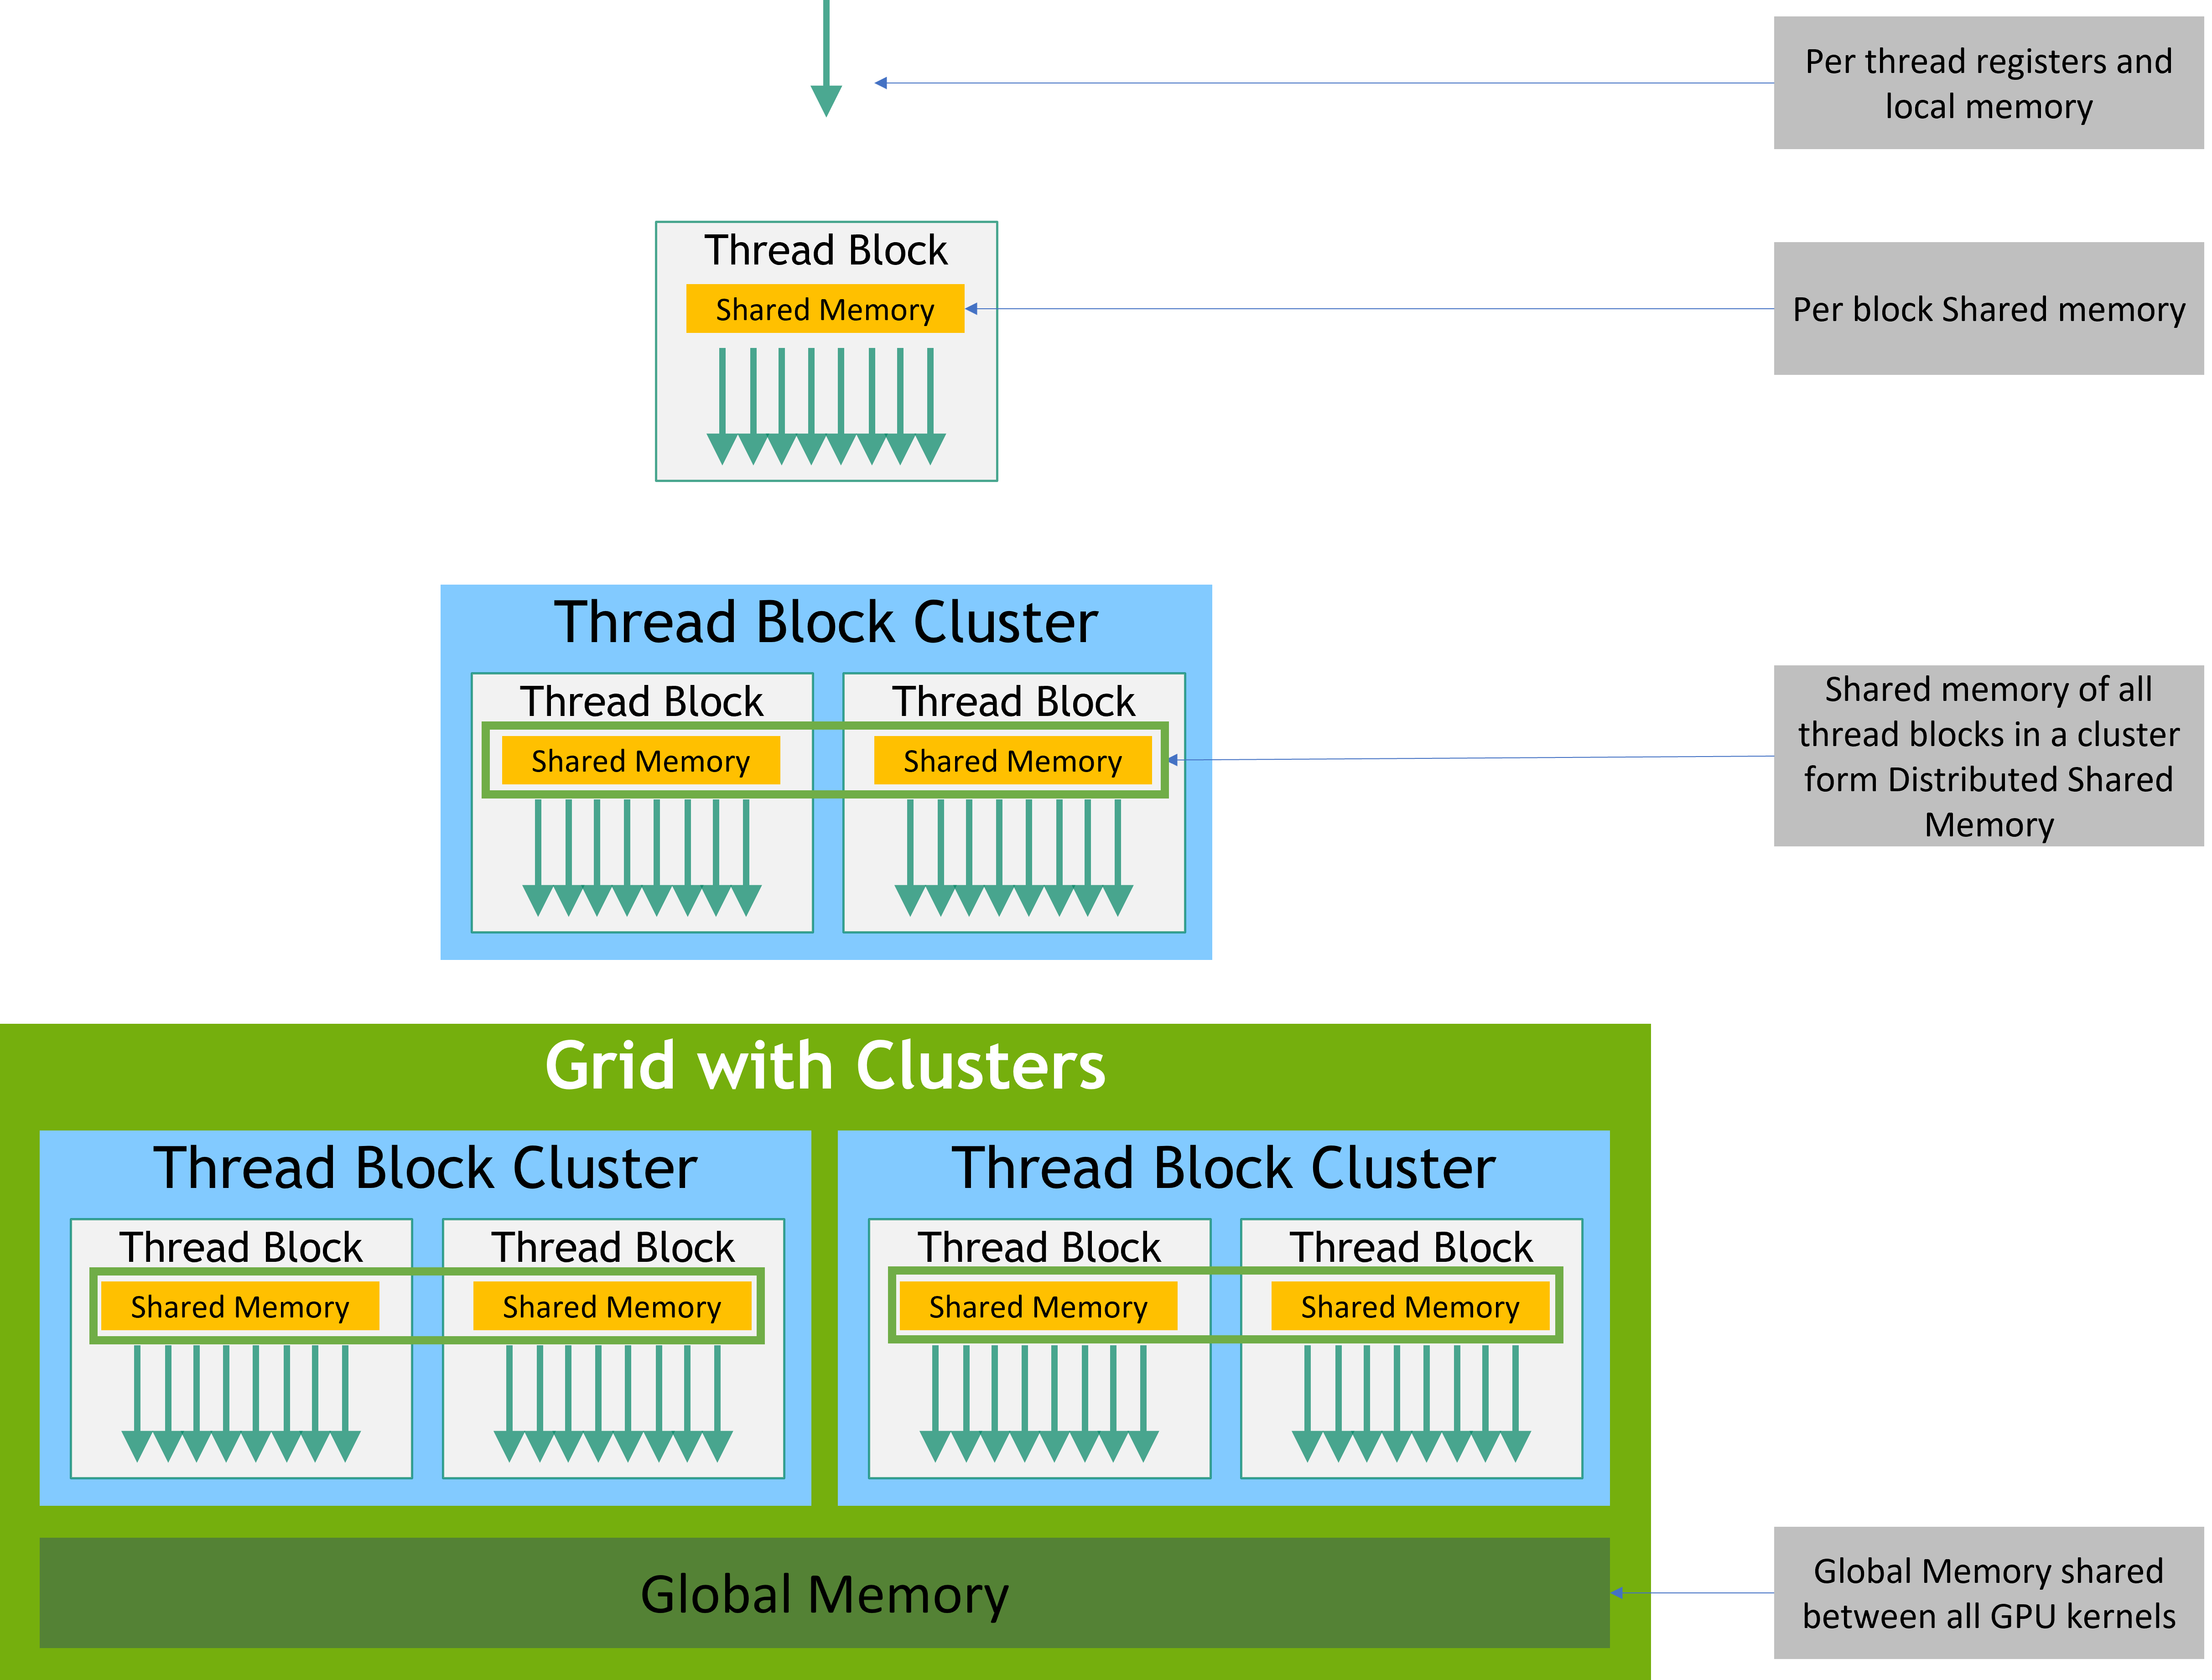
\includegraphics[scale=0.4]{src/images/memory-hierarchy.png}
    \caption{Иерархия памяти CUDA}
    \label{fig:memory_hierarchy}
\end{figure}

Программная-аппаратная модель CUDA позволяет запускать программу, написанную на языке CUDA C++, на графическом процессоре.
CUDA C++ является расширением языка C++, который позволяет объявлять C++ функции, называемые CUDA kernel,
которые будут запущены и исполнены N разными CUDA thread (далее CUDA поток). CUDA поток - это элементарная единица исполнения программы на
графическом процессоре. Ограниченный набор потоков (на данный момент, обычно до 1024) группируются в блоки (threadblock).
Каждый блок не зависит от других блоков и порядок исполнения блоков определяется аппаратной частью графического процессора, при этом каждый блок
исполняется на одном Streaming Multiprocessor (SM). Streaming Multiprocessor - это часть графического процессора, которая является
аналогом ядра в многоядерном центральном процессоре.
Блоки группируются в сетку (grid), при этом количество блоков в сетке ограничивается только диапазоном 32-битного индекса. Блок и сетка могут
иметь многомерную структура, например блок может содержать (x, y) потоков.

Важной частью программно-аппаратной модели является иерархия памяти (см. рис. \ref{fig:memory_hierarchy}). Каждый поток имеет свой собственный
набор регистров. Регистр является наиболее быстрой памятью, доступной графическому процессору. Обычно регистровый файл достаточно большой и может
содержать 255 регистров на один поток. Потоки в пределах одного блока имеют в своем распоряжении общую память (shared), которая достаточно
эффективная и является фактически программно-видимым кэшем. Обычно размеры общей памяти до 64 КБайт. Помимо этого каждый поток в каждом блоке имеет
доступ к участку оперативной памяти графического процессора, которая называется глобальная память (global). Глобальная память может достигать
размеров нескольких десятков ГБайт.

\subsection{Фреймворк машинного обучения PyTorch}
PyTorch является одним из самых часто используемых фреймворков машинного обучения \cite{pytorch_2025}\cite{pytorch_review_2024}. Это проект с открытым исходным кодом,
написанный на Python и C++, который применяется для разработки и обучения нейронных сетей. PyTorch поддерживает различные архитектуры,
в том числе центральные процессоры, графические процессоры, поддерживающие CUDA и мобильные устройства.
PyTorch содержит большое количество алгоритмов, которые используются в машинном обучении. Самые основные и важные алгоритмы являются:
\begin{itemize}
    \item операции матричного умножения
    \item операции свертки
    \item векторные/тензорные операции (сложение, скалярное произведение и т.д.)
\end{itemize}
Помимо этого, PyTorch предоставляет готовые архитектуры нейронных сетей для решения различных задач машинного обучения, например,
распознавание изображений, классификация текста и т.д.

Хоть PyTorch содержит реализации многих алгоритмов машинного обучения, Pytorch гораздо чаще использует реализации из
сторонних библиотек. Например, операции матричного умножения могут быть реализованы в библиотеке
cuBLAS \cite{cublas_2025}, операции свертки - в библиотеке cuDNN \cite{cudnn_2025} и т.д.
% В ходе исследования (см. раздел 2) было получено, что для большого числа задач PyTorch использует две библиотеки: cuBLASLt и cuDNN.
% Реализации этих библиотек является основной задачей исследования.

\subsection{CUTLASS}
Среди библиотек с открытым исходным кодом, которые могут быть использованы для реализации высокопроизводительных алгоритмов матричного умножения
и свертки особого внимания заслуживает библиотека CUTLASS \cite{cutlass_2025}.
Библиотека CUTLASS (CUDA Template Linear Algebra Subroutines) – это высокопроизводительная коллекция шаблонов и компонентов
для линейной алгебры на CUDA, разработанная NVIDIA. Она предоставляет оптимизированные реализации матричных операций
(GEMM – General Matrix Multiplication), сверток и других вычислений, используемых в глубоком обучении и
высокопроизводительных вычислениях (HPC). CU\-TLASS позволяет разработчикам создавать эффективные CUDA kernel,
используя готовые модули, что упрощает оптимизацию вычислений для различных аппаратных возможностей (например, тензорных ядер).

На момент написания данной работы библиотека CUTLASS версиии 4.0.0. Библиотека CUTLASS имеет фундаментально разные решения задач матричного
умножения и свертки в зависимости от версии. Наиболее значимые изменения свазяны с версиями 2.x и 3.x. Ввиду этого в данном обзоре будут рассматриваться
только версии CUTLASS 2.x и 3.x. Заметим, что CUTLASS является обратно совместимой с предыдущими версиями, поэтому несмотря на то, что версии 2.x и 3.x
являются более старыми, ключевые принципы организации библиотеки остаются прежними.

\subsubsection{Организация матричного умножения}
CUTLASS использует механизм шаблонов C++ для создания универсальных функций, которые могут быть использованы для реализации различных алгоритмов.
На рис. \ref{fig:cutlass_gemm} представлены основные компоненты матричного умножения для CUTLASS 2.x. Организация матричного умножения является иерархической,
что верно для большинства интерфейсов в CUTLASS. Каждый уровень организации обычно представлен каким-то шаблоном и реализует задачу своего уровня. Например,
самый нижний уровень, который называется уровнем инструкции (instruction-level) реализует примитивную операция умножения со сложение (matrix-multiply-add).
Иерархическая организация вычислений в CUTLASS соответствует модели параллелизма архитектуры CUDA и включает следующие основные уровни:
\begin{itemize}
    \item Уровень инструкции (instruction-level) — реализует примитивные операции с учетом аппаратных возможностей (например, операции умножения со сложением multiple-add)
    \item Уровень потока (thread-level) — реализует операции в рамках потока, например, работу с регистровым файлом
    \item Уровень варпа (warp-level) — реализует операции в рамках группы потоков, например, обход (iteration) матриц
    \item Уровень блока (block-level) — реализует операции в рамках блока, например, работу с глобальной памятью и общей памятью
\end{itemize}

Уровни выше, не упомянутые в списке, выполняют достаточно тривиальные операции по запуску CUDA kernel, например, выбор размер блока и
общей памяти. Стоит отметить, что эти уровни не предполагают никаких эвристик по подбору оптимальных параметров, и полностью зависят от
выбора программиста.

Так, каждый уровень выполняет какую-то конкретную задачу, например уровень блока грузит данные из
глобальной памяти в общую память соотвествующего размера, приэтом вышестоящий уровни вызывают операции уровней ниже.
Так как большинство уровней используют шаблоны, то они могут быть использованы для реализации различных алгоритмов на каждом уровне
иерархии.

\begin{figure}
    \centering
    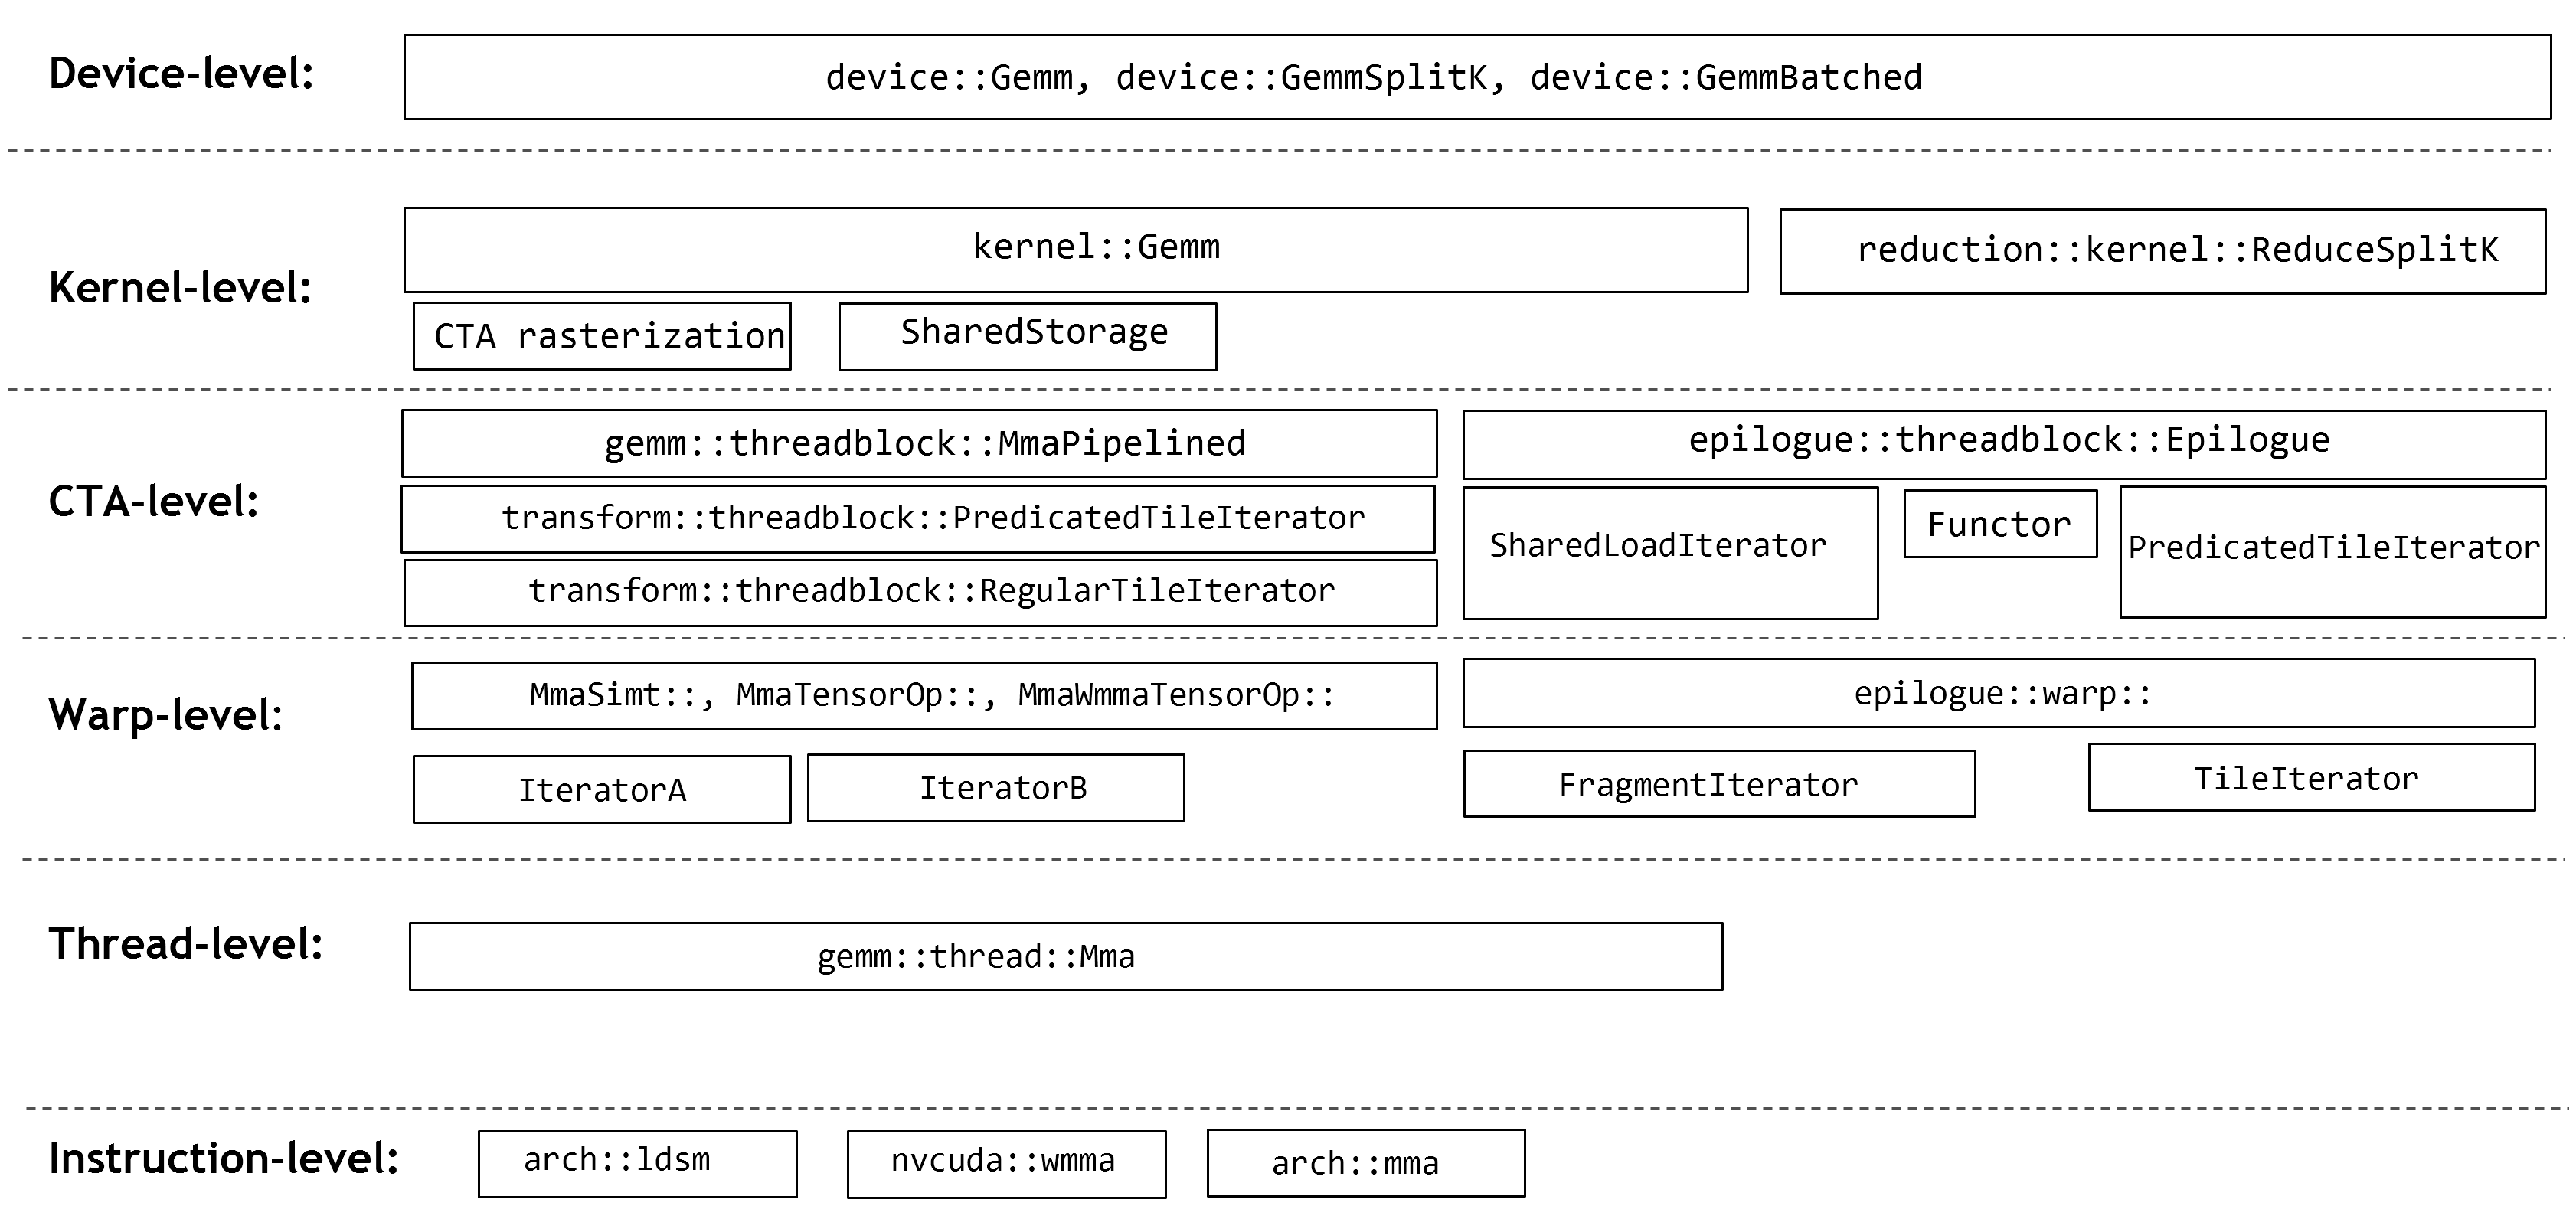
\includegraphics[scale=0.45]{src/images/cutlass-gemm-components.png}
    \caption{Основные компоненты матричного умножения для CUTLASS 2.x}
    \label{fig:cutlass_gemm}
\end{figure}


В CUTLASS 3.x основные компоненты матричного умножения представлены на рис. \ref{fig:cutlass_gemm_3.x}. В отличии от версии 2.x, где организация
полагалась на иерархию параллелизма CUDA, CUTLASS 3.x вместо этого реализует алгоритмы которые являются более универсальными и предоставляет следующие
уровни организации:
\begin{itemize}
    \item Атомарный уровень (atom-level) — реализует примитивные операции копирования (например, 64-битного числа)
    \item Уровень под-тензора (tile-level) — реализует операции в рамках под-тензора, например, копирование и умножение под-тензоров
    \item Коллективный уровень (collective-level) — является коллекцией примитов с более низких уровней, которая реализует непосредственно алгоритм матричного умножения
\end{itemize}
Самые верхние уровни, как и раньше, настраивают размеры блоков, размеры общей памяти и т.д. Такая организация позволяет сосредотачивать усилия
на реализации конкретных алгоритмов, полагаясь на оптимизированные реализации предоставляемые CUTLASS. Ключевую роль в этой организации играет
библиотека CUTE, которая позволяет описывать алгоритмы на основе примитивных операций, например, копирования, требуя меньше усилий по ансамблированию
потоков CUDA.

\begin{figure}
    \centering
    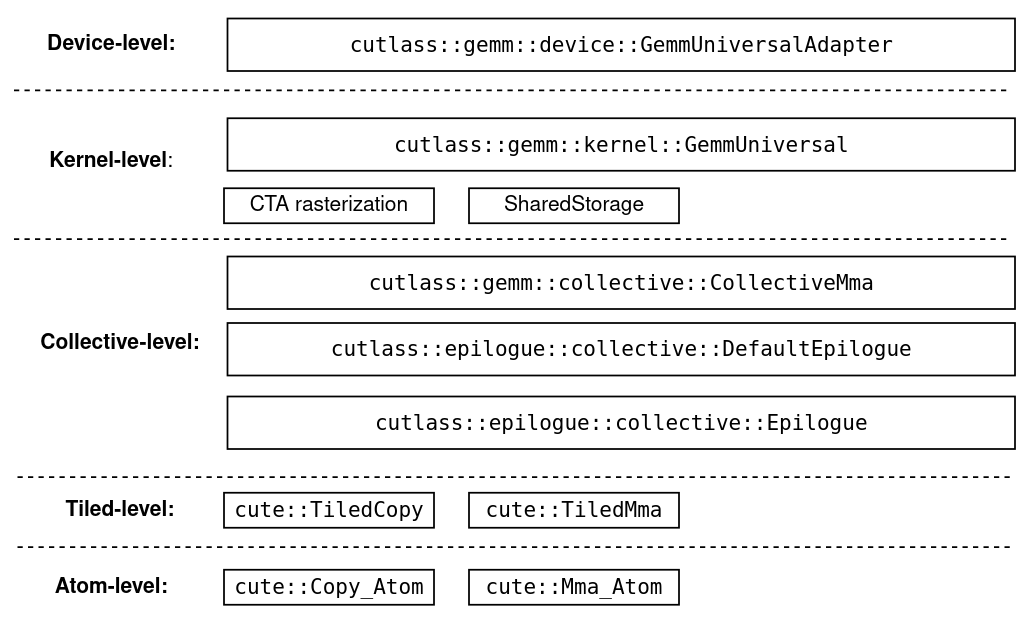
\includegraphics[scale=0.5]{src/images/cutlass-gemm3-components.png}
    \caption{Основные компоненты матричного умножения для CUTLASS 3.x}
    \label{fig:cutlass_gemm_3.x}
\end{figure}

\subsubsection{Библиотека CUTE}
В архитектуре CUTLASS 3.x ключевую роль играет библиотека CUTE, предоставляющая абстракции для реализации высокоэффективных
вычислительных алгоритмов. Данная библиотека позволяет абстрагироваться от сложностей параллельной модели выполнения CUDA.
Ключевой компонентой библиотеки CUTE является \textit{способ хранения} (далее layout), который представляет собой математические отображение:
$f \colon \mathbb{N}^n \to \mathbb{N}, где n \geq 1$, преобразующая n-мерные логические координаты в линейный индекс памяти.
Layout имеет понятие размера, то есть числа элементов, которые могут быть отображены.  Так для матрицы $A \in \mathbb{R}^{I \times J}$,
где I -- число строк, J -- число столбцов, линейный индекс в памяти вычисляется как $i \times J + j$, и является
отображением $f \colon \mathbb{N}^2 \to \mathbb{N}$, причем размером layout является $I \times J$.
Хотя логические координаты матрицы A являются двумерными (номер строки и номер столбца), CUTE позволяет использовать одномерную координату,
пересчитывая эту координату в двумерную используя колексографический порядок ("справа-налево").
Например, в случае матрицы A схема перевода будет следующая: 0 $\mapsto$ (0, 0), 1 $\mapsto$ (1, 0), 2 $\mapsto$ (2, 0), ... I $\mapsto$ (I, 0),
I + 1 $\mapsto$ (0, 1), I + 2 $\mapsto$ (1, 1), ... I $\times$ J $\mapsto$ (I, J).

Для layout реализованы операции \textit{слияния} (coalescing), \textit{композиции} (composition) и \textit{дополнения} (complement).
Операция слияния упрощает пересчет логических координат в линейный индекс, посредством упрощения формулы перевода координат.
Например, для вырожденного трехмерного массива $T \in \mathbb{R}^{K \times 1 \times M}$, операция слияния уменьшает размерность задачи,
сохряняя правильное отображение. Библиотека CUTE имеет множество статических проверок свойств отображений и позволяет упрощать вычисления
свазянные с layout, что имеет решающую роль в виду высокой цены вычислений такого рода операций на GPGPU.

Операция композиции позволяет объединить два отображения $f_1 \colon \mathbb{N}^n \to \mathbb{N}$ и $f_2 \colon \mathbb{N}^k \to \mathbb{N}$
в одно отображение $f_1 \circ f_2 \colon \mathbb{N}^m \to \mathbb{N}$, такое, что $f_1 \circ f_2(x) =$ $f_1$($f_2$(x)), где x -- логические
координаты отображения $f_2$ (не более чем k-мерный вектор). Такая композиция возможна, потому что как уже отмечалось выше, в CUTE можно вместо логических
координат использовать координаты меньше размерности, пересчитывая их в логические используя колексографический порядок. Композиция крайне полезная
операция, которая используется для того, чтобы делить массивы на подмассивы. Действительно, по определению композиции мы используем логических координаты
отображения $f_2$, которая затем переводится в логические координаты отображения $f_1$. Однако, не сложно понять, что при операции композиции мы можем
перебрать не все логические координаты $f_1$, что означает что мы обращаемся не по каждому линейному индексу в памяти. Для этого была введена операция
дополнения.

Операция дополнения можно описать как отображение $f^*$, такое что $f^*(i) \neq f(j)$, причем $0 \leq i \leq I$, и $0 \leq j \leq J$, а I + J = K, где
K какое-то конечное натуральное число. Такого рода операция полезна, когда мы обращаемся к подмассиву в каком-то массив, используя операцию композиции,
но приэтом не обращаемся ко всем элементам этого массива. Тогда дополнение будет такой layout, который будет обращаться только к тем элементам,
которые не доступны через композицию. Таким образом, через введенные три операции решается сложная задача по делению массива на подмассивы,
которая имеет решающее значение в виду высокой параллельности GPGPU и необходимости распределения вычислений по потокам.

\subsubsection{Организация свертки}
Свертка является операцией над многомерными массивами (чаще называемые тензорами). Рассмотрим наиболее распостранненый случай 4-мерных тензоров:
\begin{equation}
\label{eq:conv}
y[n,p,q,k] = \sum_{c=0}^{C-1} \sum_{r=0}^{R-1} \sum_{s=0}^{S-1} x[n, \tilde{h}(p,r), \tilde{w}(q,s), c] \cdot w[k,c,r,s]
\end{equation},
где:
\begin{itemize}
    \item $\mathbf{x} \in \mathbb{R}^{N \times H \times W \times C}$ -- входной тензор (батч изображений)
    \item $\mathbf{w} \in \mathbb{R}^{K \times C \times R \times S}$ -- тензор фильтров
    \item $\mathbf{y} \in \mathbb{R}^{N \times P \times Q \times K}$ -- выходной тензор
\end{itemize}

Координаты $\tilde{h}$ и $\tilde{w}$ определяются следующим образом:
\begin{align}
\tilde{h}(p,r) &= p \cdot s_h - p_h + r \cdot d_h \label{eq:coord_transform_h} \\
\tilde{w}(q,s) &= q \cdot s_w - p_w + s \cdot d_w \label{eq:coord_transform_w}
\end{align}

Параметры свертки:
\begin{itemize}
    \item $s_h, s_w$ -- шаг свертки (stride)
    \item $p_h, p_w$ -- дополнение (padding)
    \item $d_h, d_w$ -- коэффициент расширения (dilation)
\end{itemize}

Представленная формула \eqref{eq:conv} описывает наиболее распространённый случай двумерной свертки для четырёхмерных тензоров.
Однако, операция свертки может быть обобщена на тензоры произвольной размерности.

Операция свертки, также как и матричного умножения имеет иерархическую структуру. В библиотеке CUTLASS методом расчета свертки является
сведение его к матричному умножению (метод \textit{implicit GEMM convolution}), поэтому иерархия операций свертки аналогично иерархии операций
матричного умножения, с поправкой на то, что классы реализующие операцию свертки имеют другое имя (см. рис. \ref{fig:cutlass_gemm} и рис.
\ref{fig:cutlass_gemm_3.x}). Данный метод расчета используется преимущественно для четырёхмерных тензоров. Для данных тензоров есть два наиболее
распостряненных формата: NCHW и NHWC. Здесь N -- количество изображений, C -- количество каналов, H -- высота изображения, W -- ширина изображения.
Форматы NCHW и NHWC являются способами хранения многомерного массива в линейной памяти, приэтом названия форматов описывают порядок координат.
На данный момент, расчет свертки в CUTLASS через матричного умножения реализован только для формата NHWC. Идея расчета заключается в сведении 4-мерных
тензоров в 2-мерные матрицы А, B C по следующей схеме: $\mathbf{x}$[N, H, W, C] $\mapsto$ A[NPQ, RSC], $\mathbf{w}$[K, C, R, S] $\mapsto$ B[RSC, K],
$\mathbf{y}$[N, P, Q, K] $\mapsto$ C[NPQ, K] (см. рис. \ref{fig:implicit_gemm_algo}). Таким образом, свертка сводится к задаче матричного умножения
вида:
\begin{equation}
\mathbf{C}[\tilde{m}, \tilde{n}] = \mathbf{A}[\tilde{m}, \tilde{k}] \cdot \mathbf{B}[\tilde{k}, \tilde{n}],
\end{equation},
где:
\begin{align}
&0 \leq \tilde{m} \leq \tilde{M} = N \cdot P \cdot Q, \\
&0 \leq \tilde{n} \leq \tilde{N} = K, \\
&0 \leq \tilde{k} \leq \tilde{K} = R \cdot S \cdot C.
\end{align}

\begin{figure}
    \centering
    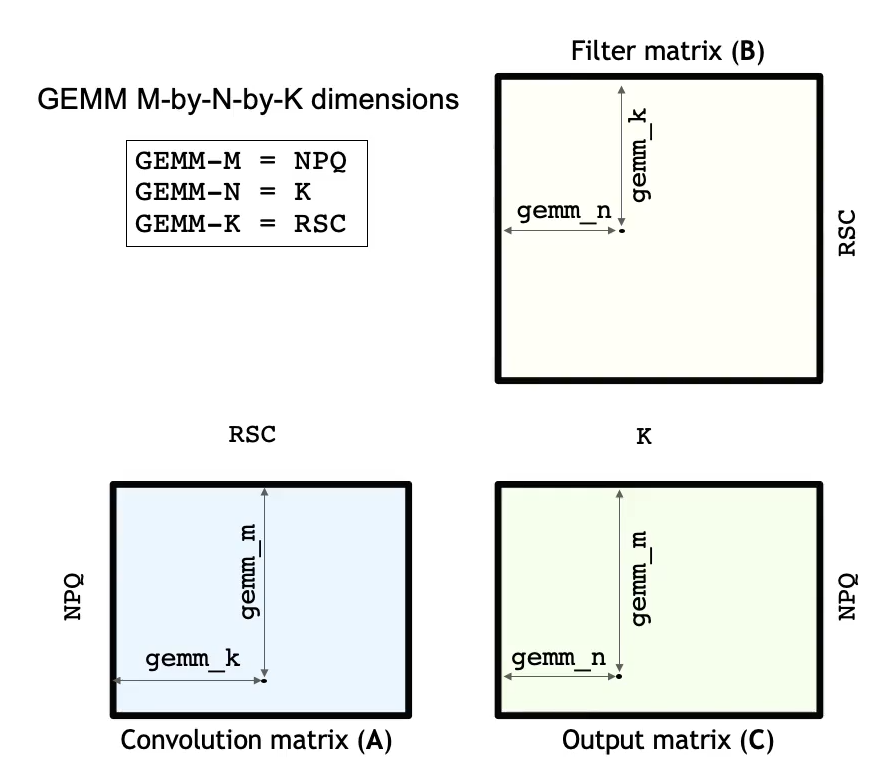
\includegraphics[scale=0.5]{src/images/implicit_gemm_algo.png}
    \caption{Сведение операции свертки к матричному умножению}
    \label{fig:implicit_gemm_algo}
\end{figure}

Важно, что такое сведение не предполагает выделение допольнительной памяти, а только пересчет координат из 4-мерного тензора в 2-мерную матрицу.
Таким образом, можно использовать эффективные алгоритмы матричного умножения для ускорения расчета свертки, но приэтом нужно тратить вычислительные
ресурсы на пересчет координат. Для решения этой задачи CUTLASS переиспользует большую часть кода для матричного умножения.
Структурно CUTLASS 2.x меняет только схему загрузки данных из глобальной памяти в общую память, остальная же часть остается прежней
(см. рис. \ref{fig:implicit_gemm_struct} -- здесь зеленым цветом обозначены измененные части по сравнению с матричным умножением).
\begin{figure}
    \centering
    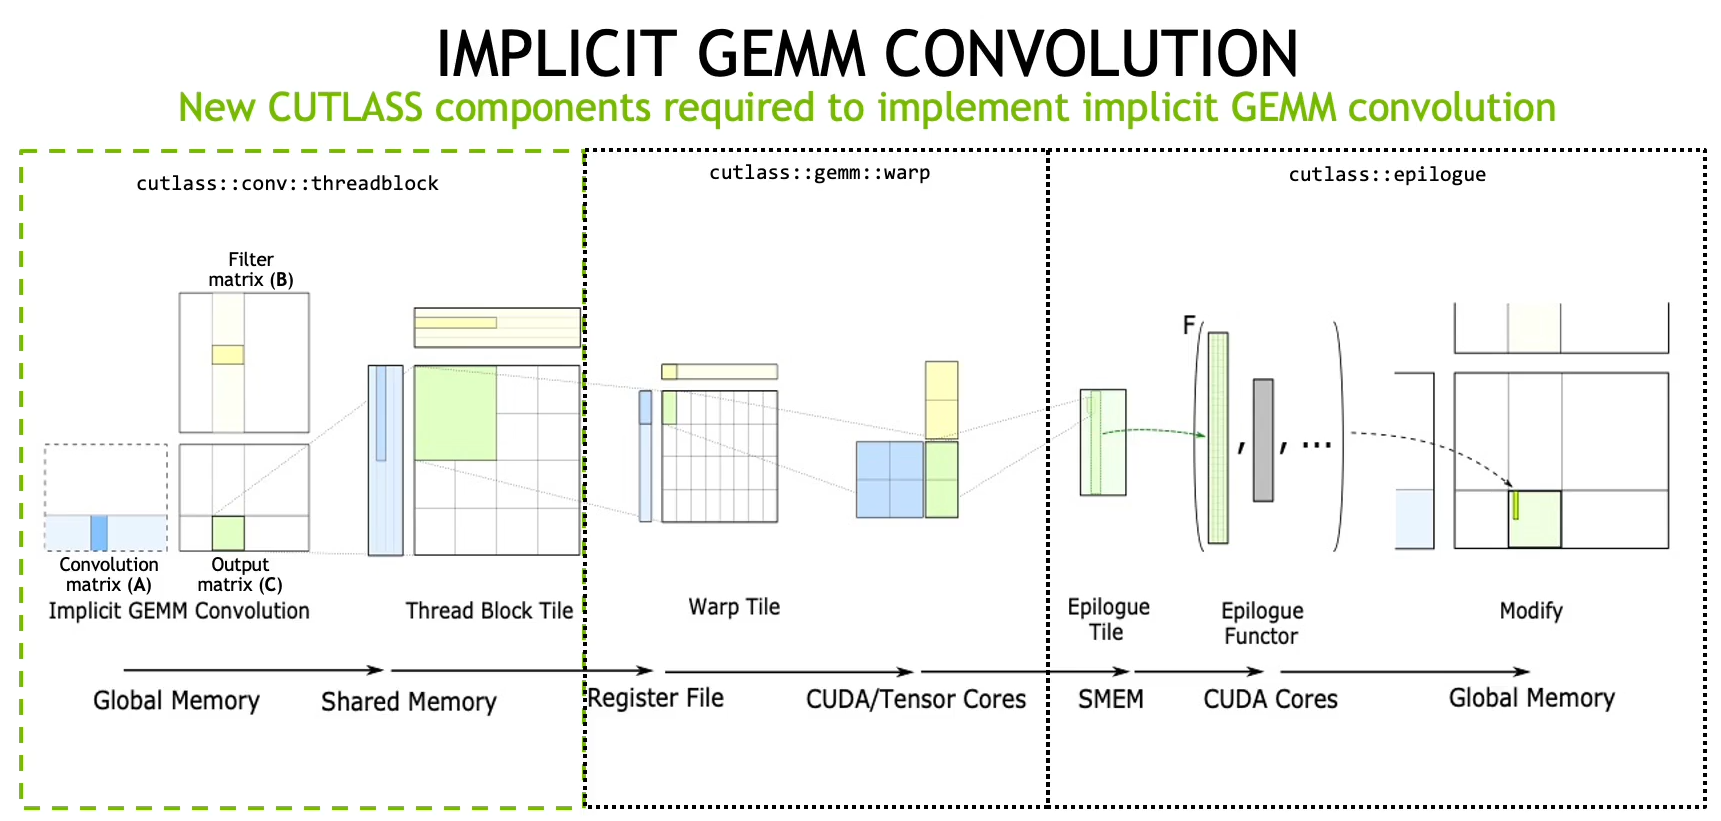
\includegraphics[scale=0.35]{src/images/implicit_gemm_struct.png}
    \caption{Структура метода расчета свертки через матричное умножение}
    \label{fig:implicit_gemm_struct}
\end{figure}

\subsubsection{Сравнение с библиотеками cuBLAS и cuDNN}
\label{subsec:comparison}

Библиотека CUTLASS демонстрирует высокую производительность при решении задач линейной алгебры и машинного обучения, однако обладает рядом
ограничений по сравнению с cuBLAS и cuDNN. Наиболее существенными являются:
\begin{enumerate}
\item \textbf{Автоматизация выбора алгоритмов}:
\begin{itemize}
\item В CUTLASS разработчик должен вручную выбирать и настраивать параметры алгоритмов
\item Библиотеки cuBLAS и cuDNN предоставляют автоматический выбор оптимальных реализаций на основе:
\begin{itemize}
\item Параметров задачи (размерности матриц/тензоров)
\item Аппаратных характеристик GPU
\item Требуемой численной точности
\end{itemize}
\end{itemize}

\item \textbf{Степень поддержки операций машинного обучения}:
    \begin{itemize}
    \item Отсутствие поддержки NCHW для совместимости с PyTorch
    \item Отсутствие реализации пакетной нормализации
    \end{itemize}
\end{enumerate}

Особую важность представляет поддержка формата NCHW, который является стандартом де-факто в большинстве фреймворков машинного обучения, включая PyTorch.
Отсутствие этой функциональности существенно ограничивает применимость CUTLASS в промышленных решениях.

Менее критичным ограничением является более низкие показатели производительности. В разделе \ref{sec:survey} показано, что CUTLASS в задачах матричного умножения
достигает 90-95\% производительности cuBLAS. Для создания полноценной аналогов cuBLAS и cuDNN необходимо разработать систему автоматического выбора алгоритмов,
расширить поддержку операций машинного обучения и провести оптимизацию алгоритмов.